\subsection{Analysis of Vulnerable domains}
\vspace{-1.5ex}
We performed the following analyses on the domains that were found to contain \ehi vulnerability:
\begin{itemize}
	\item Checking Alexa rankings of the vulnerable domains.
	\item Investigating the back-end languages used by the vulnerable domains.
%	TODO Adam: Should these abbreviations be expanded here or further down where we explain?
	\item Analyzing the presence of DKIM~\cite{allman2007domainkeys}, SPF~\cite{schlitt2006sender}, and DMARC~\cite{kucherawy2015domain} mechanisms on these domains.
\end{itemize}

\vspace{-1.5ex}
\subsubsection{Alexa rankings of vulnerable domains.}
We searched through the Alexa rankings data\cite{alexa} for the domains that were found to be vulnerable, and found 135 of these domains in the top 1 million ranked websites, with 1 website in the top 5,000, and 4 in the top 20,000. A detailed distribution of the rankings is shown in Figure~\ref{fig:alexa_data_bar} and Figure~\ref{fig:alexa_data_pie}.

%TODO Adam: Need to decide if table or graph, if graph, then Pie vs Bar.
%\begin{table}[tbp]
%	\centering
%	\scriptsize
%	\begin{tabular}{|l|c|}
%		\hline
%		\textbf{Alexa Ranking Ranges} & \textbf{Vulnerable domains} \\
%		\hline
%		0-5K & 1 \\
%		\hline
%		5-50k & 7 \\
%		\hline
%		50k-100k & 6 \\
%		\hline
%		100k-250k & 23 \\
%		\hline
%		250k-500k & 30 \\
%		\hline
%		500k-1m & 68 \\
%		\hline		
%	\end{tabular}
%	\caption[\titlecap{Distribution of vulnerable domains based on Alexa Rankings}]{Distribution of vulnerable domains based on Alexa Rankings}
%	\vspace{-5ex}
%	\label{tab:alexa}
%\end{table}

\begin{figure}
	\centering
	\begin{minipage}{.5\textwidth}
		\centering
		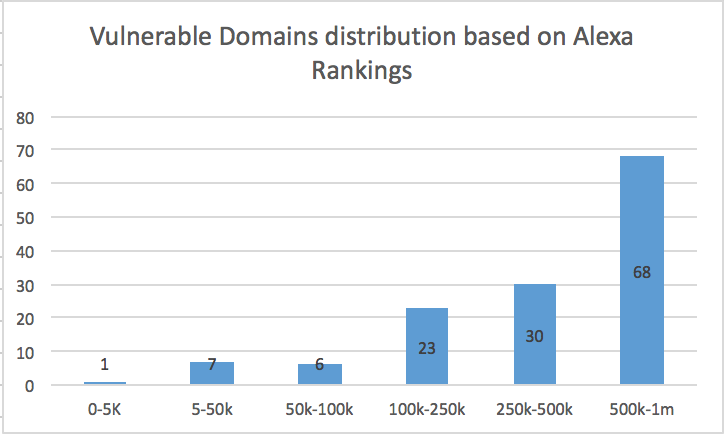
\includegraphics[width=.95\linewidth]{alexa_data_bar}
		\captionof{figure}{Distribution of vulnerable domains based on Alexa Rankings}
		\label{fig:alexa_data_bar}
	\end{minipage}%
	\begin{minipage}{.5\textwidth}
		\centering
		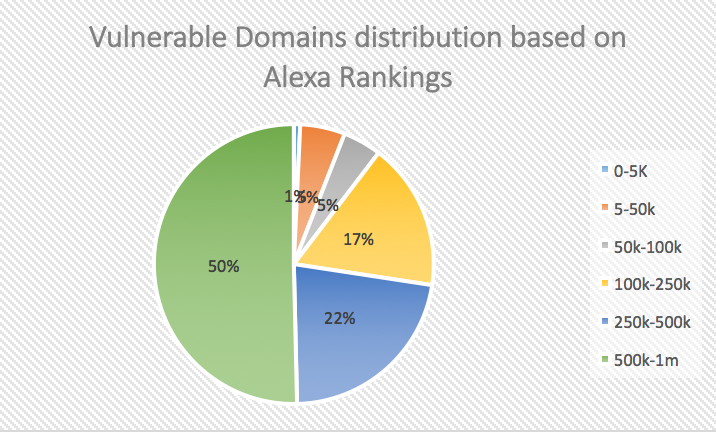
\includegraphics[width=.95\linewidth]{alexa_data_pie}
		\captionof{figure}{Distribution of vulnerable domains based on Alexa Rankings}
		\label{fig:alexa_data_pie}
	\end{minipage}
	\vspace{-1.5ex}
\end{figure}
\vspace{-1.5ex}

%TODO Adam: Is a table/graph for backend technologies needed?
% apparently \subsubsection need to have a period at the end.
\subsubsection{Back-end technologies of vulnerable domains.}
We investigated the top 100 vulnerable domains on our list (based on the alexa rankings) to find the back-end technologies used by these vulnerable domains to see if there was any recurring pattern. Using BuiltWith~\cite{builtwith} and Wappalyzer~\cite{wappalyzer}, we found that a majority of the vulnerable domains (79\%) used PHP as one of the back-end technologies, while 17\% of domains used WordPress and another 14\% used ASP.Net. Other technologies used include Java (5\%), Ruby on Rails (1\%), and Perl (1\%). We also found a combination of other technologies like Magento, CakePHP, CodeIgniter, Joomla, mail.ru and Drupal being used in conjunction with one of the above languages. A point to be noted is that 4\% of the websites also used Contact Form 7~\cite{CF7}, which is supposed to protect against such attacks.

%\begin{wraptable}{r}{5.5cm}
\begin{table}[tbp]
	\centering
	\scriptsize
	\begin{tabular}{|l|c|}
		\hline
		Technologies used & \% of Vulnerable Domains \\
		\hline
		PHP & 79 \\
		\hline
		ASP.net & 14 \\
		\hline
		J2EE & 5 \\
		\hline
		Perl & 1 \\
		\hline
		Ruby on Rails & 1 \\
		\hline
		Wordpress & 17 \\
		\hline
	\end{tabular}
	\caption[\titlecap{Distribution of vulnerable domains based on technologies used}]{Distribution of vulnerable domains based on technologies used}
	
	\label{tab:lang_used}
\end{table}
%\end{wraptable}

\vspace{-1.5ex} 
\subsubsection{Presence of e-mail spoofing protection on vulnerable domains.}
We investigated the presence of anti-spoofing mechanisms such as DKIM (DomainKeys Identified Mail), SPF (Sender Policy Framework), and DMARC (Domain-based Message Authentication, Reporting \& Conformance) in the vulnerable domains. Protection mechanisms such as these make it harder for an attacker to spoof the \email messages from these domains manually by forging the \texttt{From} addresses of \emails.

Out of the top 100 vulnerable domains on our list (based on the alexa rankings), we found that SPF protection was present on 71 of these websites, DKIM on 59 of these websites, and DMARC on 7 of these websites.

This makes \ehi attacks all the more effective as now we have a way to spoof messages from domains that have anti-spoofing mechanisms in place preventing manual spoofing.